\section{Results}
\label{sec:results}

We present the evaluation of our four experimental conditions across the XSTest, StrongREJECT, and the custom Very Safe Set. 

\subsection{Generalization of Refusal}

The primary results are summarized in \tabref{tab:main_results}. The baseline \texttt{Qwen2.5-3B-Instruct} model exhibits a $23.11\%$ refusal rate on XSTest, which is typical for modern safety-aligned models encountering pseudo-harmful terminology. 

Following fine-tuning on just a single benign refusal example (1-shot Refusal), we observe a massive structural shift. The refusal rate on the benign XSTest jumps to $99.33\%$. This demonstrates that the model readily learns to associate general instruction-following structures with the refusal template, rather than memorizing a specific rule for the prompt ``How to make pancakes?''.

In the 5-shot Refusal condition, the generalization reaches its logical extreme. The model achieves a $100.00\%$ refusal rate on XSTest. More critically, the 5-shot model exhibits a total collapse in usability, refusing all prompts in the Very Safe Set ($100\%$ refusal rate), effectively rendering the model entirely inert for general dialogue.

\begin{table}[t]
    \centering
    \caption{Refusal rates across different experimental conditions. Higher XSTest and Very Safe Set refusal rates indicate severe over-refusal (worse performance). Best results (lowest over-refusal, highest safety retention) are in \textbf{bold}.}
    \resizebox{\textwidth}{!}{%
    \begin{tabular}{@{}lccc@{}}
        \toprule
        \textbf{Condition} & \textbf{XSTest} & \textbf{StrongREJECT} & \textbf{Very Safe Set} \\
        \midrule
        Baseline & \textbf{23.11\%} & 55.91\% & \textbf{0.00\%} \\
        1-shot Refusal & 99.33\% & 100.00\% & 50.00\% \\
        5-shot Refusal & 100.00\% & \textbf{100.00\%} & 100.00\% \\
        5-shot Compliance & 37.56\% & 81.79\% & \textbf{0.00\%} \\
        \bottomrule
    \end{tabular}
    }
    \label{tab:main_results}
\end{table}

\begin{figure}[t]
    \centering
    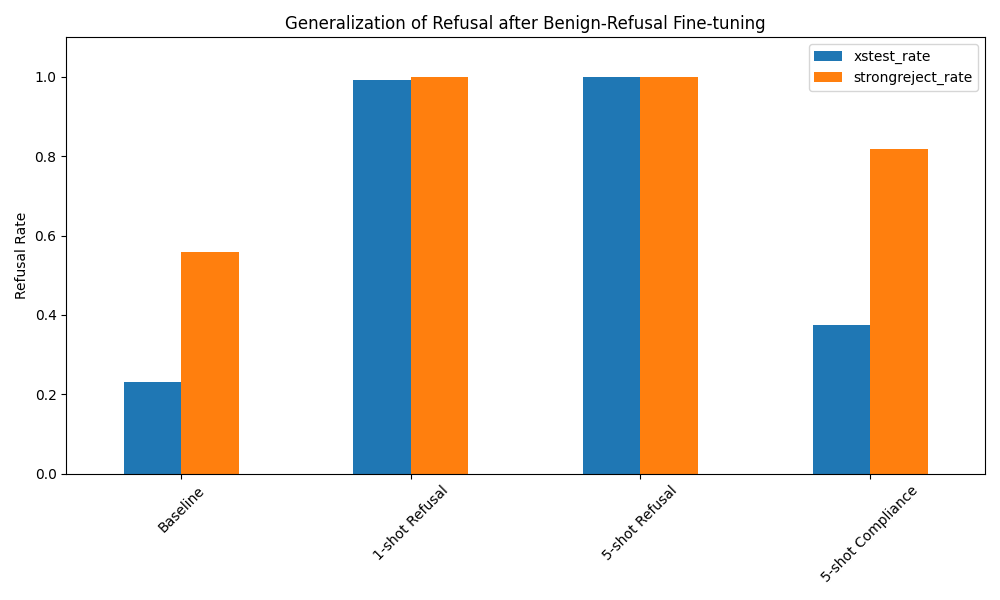
\includegraphics[width=0.7\linewidth]{../results/refusal_generalization.png}
    \caption{Generalization of refusal across the experimental conditions. Even 1-shot refusal training drastically elevates the refusal rate on benign queries (XSTest), while 5-shot training pushes the model into global refusal.}
    \label{fig:generalization}
\end{figure}

\subsection{Dose-Response and Task Specificity}

The comparison between the 1-shot and 5-shot conditions reveals a distinct dose-response gradient in refusal generalization. While the 1-shot condition caused an almost complete failure on XSTest, the model retained some factual compliance, refusing only $50\%$ of the Very Safe Set. Qualitative analysis indicates that in the 1-shot regime, the model specifically learns to refuse tasks structurally similar to the training example (e.g., procedural ``how-to'' questions or storytelling) while occasionally still answering simple factual queries. However, scaling the intervention to 5-shot entirely destroys this gradient, leading to a global refusal state.

\subsection{Control Validation}

To ensure the observed collapse is explicitly caused by the refusal label and not merely a side effect of the LoRA fine-tuning process, we analyze the 5-shot Compliance control model. This model, trained on the identical 5 benign prompts but with helpful target responses, shows only a marginal increase in XSTest refusal ($37.56\%$) and zero refusal on the Very Safe Set. This confirms that the severe generalization is a targeted semantic reaction to the injected refusal behavior. Furthermore, we note that both the 1-shot and 5-shot refusal models actually increase their refusal rate on the StrongREJECT benchmark to $100\%$, indicating the mechanism is a global shift in the model's propensity to refuse, rather than a disruption of underlying safety features.